%!TEX program = xelatex
\documentclass[UTF8]{ctexart}
    \usepackage{amsmath}
    \usepackage{geometry}
	\usepackage{graphicx}
	\usepackage[utf8]{inputenc}
    \usepackage{listings}
    \usepackage{longtable}
    \usepackage{multirow}
	\usepackage{url}
    \usepackage{verbatim}
	
	\graphicspath{ {./images/} }

    \title{给定文法的自底向上语法分析程序文档}
    \author{2016211305班 \ 熊光正 (学号:2016211249)}
\begin{document}
\lstset{numbers=left,frame=single,breaklines=true}
\maketitle
\tableofcontents
\clearpage
\section{开发环境}
本程序使用$Visual \ Studio \ Code$编辑器,为复用之前的代码,使用$C++$,在基于$x86\_64$指令集的$64$位中文$Windows \ 10$环境下开发。
程序使用$Clang++$(版本号:$7.0.0$)编译器,基于$c++14$标准和$MSVC$环境进行编译。
\section{运行环境}
本程序支持在基于$x86\_64$指令集的$64$位中文$Windows \ 10$环境下运行,没有其他运行时依赖。
\section{设计概述}
根据要求,程序输入待分析的句子,输出分析及计算结果。运行时,程序先初始化符号栈、状态栈、属性栈,后依据分析表和$SDD$执行$DFA$,并输出结果。
\section{程序实现}
\subsection{数据结构}
\begin{longtable}[c]{|c|c|c|}
    \hline
    逻辑结构 & 数据结构 & 备注 \\ \hline
    \endfirsthead
    \hline
    逻辑结构 & 数据结构 & 备注 \\ \hline
    \endhead
    (任意)符号  &  $symbol = string$ &  \\ \hline
    $DFA$状态  &  $DFAState = int$ &  \\ \hline
    句子和短语 & $deque<symbol>$  &   \\ \hline
    符号栈 & $vector<symbol>$  &   \\ \hline
    状态栈 & $vector<DFAState>$  &   \\ \hline
    属性栈 & $vector<float>$  &   \\ \hline
    分析动作类型 & $ActionType = int$  &  移进、归约等 \\ \hline
    分析动作 & $pair<ActionType, DFAState>$  &  \\ \hline
    一行分析表 & $unordered\_map<symbol, AnalyseAction>$  &  \\ \hline
    分析表 & $unordered\_map<DFAState, AnalyseTableLine>$  &  \\ \hline
    文法规则 & $Rule = pair<symbol, int>$  &  $int$为产生式长度 \\ \hline
    \caption{数据结构表}
    \label{数据结构表}\\
    \end{longtable}
\subsection{文法和$SDD$}
拓广文法并构建$SDD$
\begin{longtable}[c]{|c|c|c|}
    \hline
    序号 & 产生式      & 语义规则                                          \\ \hline
    \endfirsthead
    \hline
    序号 & 产生式 & 语义规则 \\ \hline
    \endhead
    1  & $E'→E$     & $E’.val=E.val;print(E'.val);$ \\ \hline
    2  & $E→E_1+T$ & $E.val=E_1.val+t.val;$                          \\ \hline
    3  & $E→E_1-T$ & $E.val=E_1.val-T.val;$                          \\ \hline
    4  & $E→T$      & $E.val=T.val;$                                   \\ \hline
    5  & $T→T_1*F$ & $T.val=T_1.val*F.val;$                          \\ \hline
    6  & $T→T_1/F$ & $T.val=T_1.val/F.val;$                          \\ \hline
    7  & $T→F$      & $T.val=F.val;$                                   \\ \hline
    8  & $F→(E)$    & $F.val=E.val;$                                   \\ \hline
    9  & $F→num$    & $F.val=num.lexval;$                              \\ \hline
    \caption{$SDD$}
    \label{$SDD$}\\
    \end{longtable}
    其中,$E.val,F.val,T.val$为综合属性,表示对应表达式的值;$num.lexval$为词法分析得到的数值。
\subsection{$FIRST$集和$FOLLOW$集}
\begin{longtable}[c]{|c|c|c|}
    \hline
    非终结符 & FIRST集 & FOLLOW集      \\ \hline
    \endfirsthead
    \hline
    非终结符 & FIRST集 & FOLLOW集      \\ \hline
    \endhead
    $E'$   & $(,num$  & $\$$           \\ \hline
    $E$    & $(,num$  & $\$,+,-,)$     \\ \hline
    $T$    & $(,num$  & $\$,+,-,),*,/$ \\ \hline
    $F$    & $(,num$  & $\$,+,-,),*,/$ \\ \hline
    \caption{$FIRST$集和$FOLLOW$集}
    \label{$FIRST$集和$FOLLOW$集}\\
    \end{longtable}
\subsection{DFA}
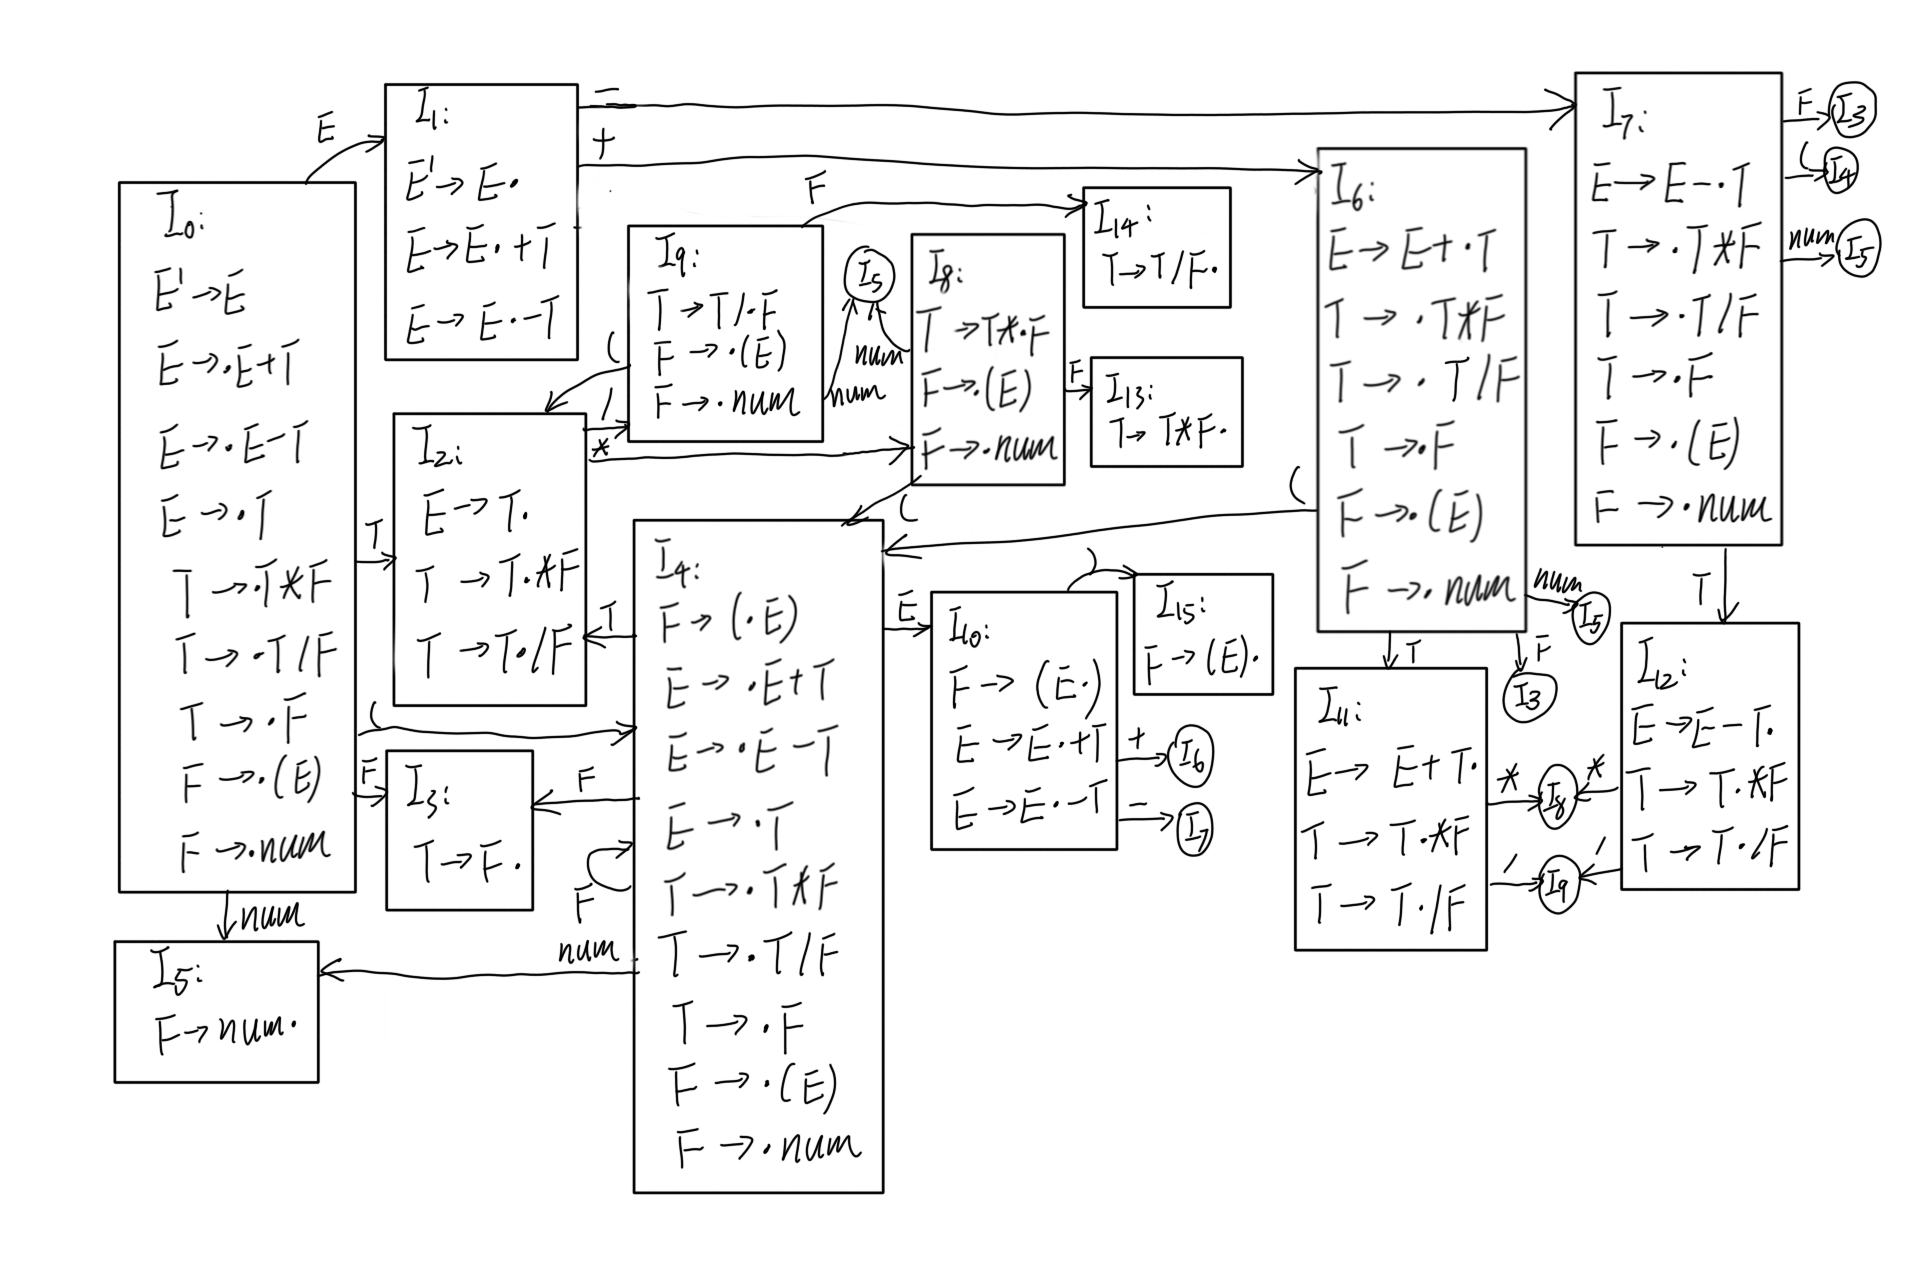
\includegraphics[width=\textwidth]{DFA}
\subsection{$SLR(1)$分析表}
\begin{longtable}[c]{|c|c|c|c|c|c|c|c|c|c|c|c|}
    \hline
    \multirow{2}{*}{状态} & \multicolumn{8}{c|}{Action}              & \multicolumn{3}{c|}{goto} \\ \cline{2-12} 
                        & +  & -  & *  & /  & (  & )   & num & \$  & E       & T      & F      \\ \hline
    \endfirsthead
    \hline
    \multirow{2}{*}{状态} & \multicolumn{8}{c|}{Action}              & \multicolumn{3}{c|}{goto} \\ \cline{2-12} 
                        & +  & -  & *  & /  & (  & )   & num & \$  & E       & T      & F      \\ \hline
    \endhead
    0                   &    &    &    &    & S4 &     & S5  &     & 1       & 2      & 3      \\ \hline
    1                   & S6 & S7 &    &    &    &     &     & ACC &         &        &        \\ \hline
    2                   & R4 & R4 & S8 & S9 &    & R4  &     & R4  &         &        &        \\ \hline
    3                   & R7 & R7 & R7 & R7 &    & R7  &     & R7  &         &        &        \\ \hline
    4                   &    &    &    &    & S4 &     & S5  &     & 10      & 2      & 3      \\ \hline
    5                   & R9 & R9 & R9 & R9 &    & R9  &     & R9  &         &        &        \\ \hline
    6                   &    &    &    &    & S4 &     & S5  &     &         & 11     & 3      \\ \hline
    7                   &    &    &    &    & S4 &     & S5  &     &         & 12     & 3      \\ \hline
    8                   &    &    &    &    & S4 &     & S5  &     &         &        & 13     \\ \hline
    9                   &    &    &    &    & S4 &     & S5  &     &         &        & 14     \\ \hline
    10                  & S6 & S7 &    &    &    & S15 &     &     &         &        &        \\ \hline
    11                  & R2 & R2 & S8 & S9 &    & R2  &     & R2  &         &        &        \\ \hline
    12                  & R3 & R3 & S8 & S9 &    & R3  &     & R3  &         &        &        \\ \hline
    13                  & R5 & R5 & R5 & R5 &    & R5  &     & R5  &         &        &        \\ \hline
    14                  & R6 & R6 & R6 & R6 &    & R6  &     & R6  &         &        &        \\ \hline
    15                  & R8 & R8 & R8 & R8 &    & R8  &     & R8  &         &        &        \\ \hline
    \end{longtable}
\subsection{翻译算法}
程序基于$S$属性定义的自底向上翻译计算表达式的值,即:
执行移进前,若输入符号为数字,将其$lexval$压入属性栈,否则将占位符压入属性栈;
执行归约前,先执行$SDD$中定义的代码段。
\section{输入输出说明}
程序可以交互式地从控制台接受用户输入,也可在运行时指定文件名,从文件自动读入,并输出至控制台。
\subsection{交互式运行}
根据程序输出的提示,用户输入待分析的句子,各符号以空格分隔,句子以换行符结束。
\subsection{从文件读取输入}
程序检查启动参数,若存在启动参数,即指定了输入文件的文件名,则从该文件中读取输入,文件格式与交互式运行时的输入格式一致。
\section{测试样例说明}
\subsection{标准测试样例集:$sample\_1.txt$}
\begin{lstlisting}
1 - 2 * 3 + 6 / 4

    \end{lstlisting}
将$sample\_1.txt$文件拖拽至$main.exe$文件上,分析输出: \\
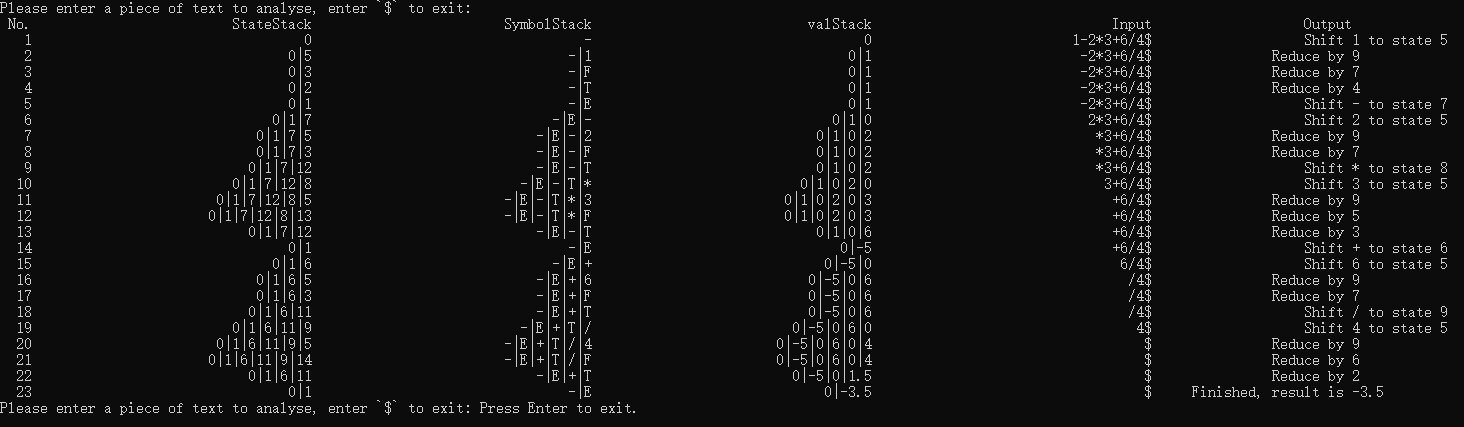
\includegraphics[width=\textwidth]{sample_1}
\begin{lstlisting}
Please enter a piece of text to analyse, enter `$` to exit:
 No.                         StateStack                        SymbolStack                           valStack                              Input                   Output
   1                                  0                                  -                                  0                         1-2*3+6/4$                   Shift 1 to state 5
   2                                0|5                                -|1                                0|1                          -2*3+6/4$               Reduce by 9
   3                                0|3                                -|F                                0|1                          -2*3+6/4$               Reduce by 7
   4                                0|2                                -|T                                0|1                          -2*3+6/4$               Reduce by 4
   5                                0|1                                -|E                                0|1                          -2*3+6/4$                   Shift - to state 7
   6                              0|1|7                              -|E|-                              0|1|0                           2*3+6/4$                   Shift 2 to state 5
   7                            0|1|7|5                            -|E|-|2                            0|1|0|2                            *3+6/4$               Reduce by 9
   8                            0|1|7|3                            -|E|-|F                            0|1|0|2                            *3+6/4$               Reduce by 7
   9                           0|1|7|12                            -|E|-|T                            0|1|0|2                            *3+6/4$                   Shift * to state 8
  10                         0|1|7|12|8                          -|E|-|T|*                          0|1|0|2|0                             3+6/4$                   Shift 3 to state 5
  11                       0|1|7|12|8|5                        -|E|-|T|*|3                        0|1|0|2|0|3                              +6/4$               Reduce by 9
  12                      0|1|7|12|8|13                        -|E|-|T|*|F                        0|1|0|2|0|3                              +6/4$               Reduce by 5
  13                           0|1|7|12                            -|E|-|T                            0|1|0|6                              +6/4$               Reduce by 3
  14                                0|1                                -|E                               0|-5                              +6/4$                   Shift + to state 6
  15                              0|1|6                              -|E|+                             0|-5|0                               6/4$                   Shift 6 to state 5
  16                            0|1|6|5                            -|E|+|6                           0|-5|0|6                                /4$               Reduce by 9
  17                            0|1|6|3                            -|E|+|F                           0|-5|0|6                                /4$               Reduce by 7
  18                           0|1|6|11                            -|E|+|T                           0|-5|0|6                                /4$                   Shift / to state 9
  19                         0|1|6|11|9                          -|E|+|T|/                         0|-5|0|6|0                                 4$                   Shift 4 to state 5
  20                       0|1|6|11|9|5                        -|E|+|T|/|4                       0|-5|0|6|0|4                                  $               Reduce by 9
  21                      0|1|6|11|9|14                        -|E|+|T|/|F                       0|-5|0|6|0|4                                  $               Reduce by 6
  22                           0|1|6|11                            -|E|+|T                         0|-5|0|1.5                                  $               Reduce by 2
  23                                0|1                                -|E                             0|-3.5                                  $     Finished, result is -3.5
Please enter a piece of text to analyse, enter `$` to exit: Press Enter to exit.
    \end{lstlisting}

\subsection{括号测试样例集:$sample\_2.txt$}
\begin{lstlisting}
( 1 - 2 ) * ( 3 + 6 ) / 4

    \end{lstlisting}
将$sample\_2.txt$文件拖拽至$main.exe$文件上,分析输出: \\
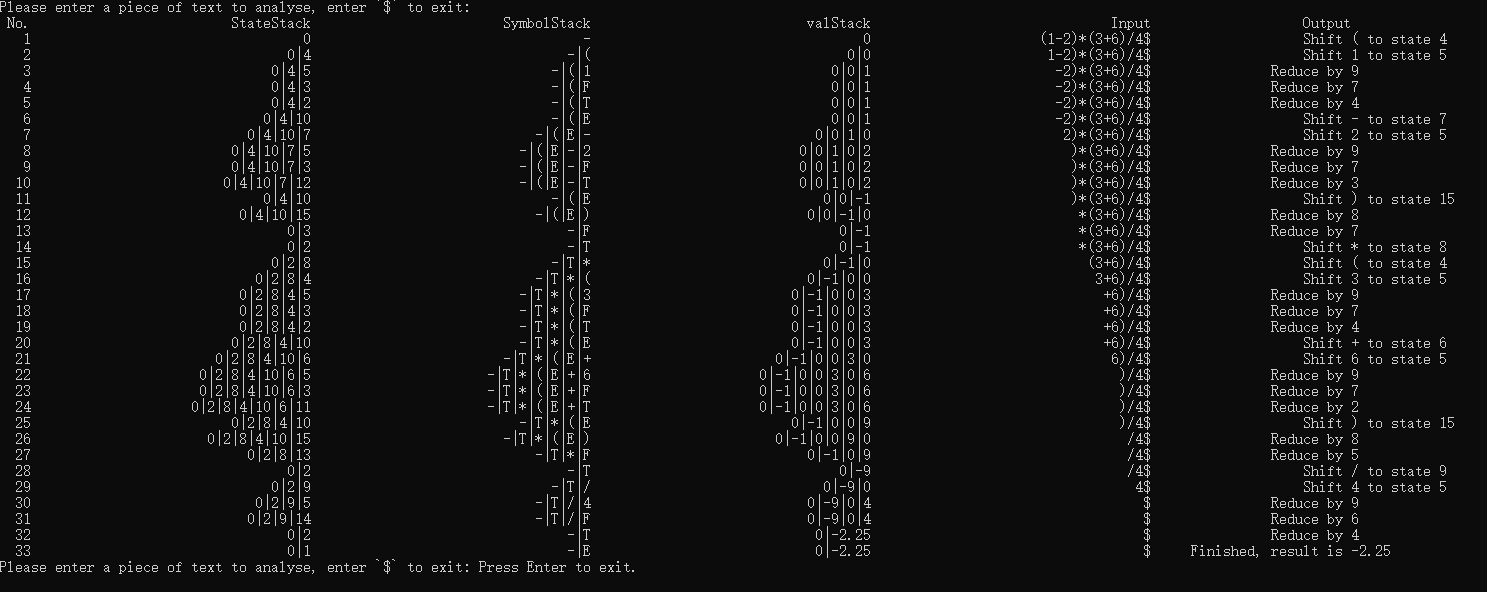
\includegraphics[width=\textwidth]{sample_2}
\begin{lstlisting}
Please enter a piece of text to analyse, enter `$` to exit:
 No.                         StateStack                        SymbolStack                           valStack                              Input                   Output
   1                                  0                                  -                                  0                     (1-2)*(3+6)/4$                   Shift ( to state 4
   2                                0|4                                -|(                                0|0                      1-2)*(3+6)/4$                   Shift 1 to state 5
   3                              0|4|5                              -|(|1                              0|0|1                       -2)*(3+6)/4$               Reduce by 9
   4                              0|4|3                              -|(|F                              0|0|1                       -2)*(3+6)/4$               Reduce by 7
   5                              0|4|2                              -|(|T                              0|0|1                       -2)*(3+6)/4$               Reduce by 4
   6                             0|4|10                              -|(|E                              0|0|1                       -2)*(3+6)/4$                   Shift - to state 7
   7                           0|4|10|7                            -|(|E|-                            0|0|1|0                        2)*(3+6)/4$                   Shift 2 to state 5
   8                         0|4|10|7|5                          -|(|E|-|2                          0|0|1|0|2                         )*(3+6)/4$               Reduce by 9
   9                         0|4|10|7|3                          -|(|E|-|F                          0|0|1|0|2                         )*(3+6)/4$               Reduce by 7
  10                        0|4|10|7|12                          -|(|E|-|T                          0|0|1|0|2                         )*(3+6)/4$               Reduce by 3
  11                             0|4|10                              -|(|E                             0|0|-1                         )*(3+6)/4$                   Shift ) to state 15
  12                          0|4|10|15                            -|(|E|)                           0|0|-1|0                          *(3+6)/4$               Reduce by 8
  13                                0|3                                -|F                               0|-1                          *(3+6)/4$               Reduce by 7
  14                                0|2                                -|T                               0|-1                          *(3+6)/4$                   Shift * to state 8
  15                              0|2|8                              -|T|*                             0|-1|0                           (3+6)/4$                   Shift ( to state 4
  16                            0|2|8|4                            -|T|*|(                           0|-1|0|0                            3+6)/4$                   Shift 3 to state 5
  17                          0|2|8|4|5                          -|T|*|(|3                         0|-1|0|0|3                             +6)/4$               Reduce by 9
  18                          0|2|8|4|3                          -|T|*|(|F                         0|-1|0|0|3                             +6)/4$               Reduce by 7
  19                          0|2|8|4|2                          -|T|*|(|T                         0|-1|0|0|3                             +6)/4$               Reduce by 4
  20                         0|2|8|4|10                          -|T|*|(|E                         0|-1|0|0|3                             +6)/4$                   Shift + to state 6
  21                       0|2|8|4|10|6                        -|T|*|(|E|+                       0|-1|0|0|3|0                              6)/4$                   Shift 6 to state 5
  22                     0|2|8|4|10|6|5                      -|T|*|(|E|+|6                     0|-1|0|0|3|0|6                               )/4$               Reduce by 9
  23                     0|2|8|4|10|6|3                      -|T|*|(|E|+|F                     0|-1|0|0|3|0|6                               )/4$               Reduce by 7
  24                    0|2|8|4|10|6|11                      -|T|*|(|E|+|T                     0|-1|0|0|3|0|6                               )/4$               Reduce by 2
  25                         0|2|8|4|10                          -|T|*|(|E                         0|-1|0|0|9                               )/4$                   Shift ) to state 15
  26                      0|2|8|4|10|15                        -|T|*|(|E|)                       0|-1|0|0|9|0                                /4$               Reduce by 8
  27                           0|2|8|13                            -|T|*|F                           0|-1|0|9                                /4$               Reduce by 5
  28                                0|2                                -|T                               0|-9                                /4$                   Shift / to state 9
  29                              0|2|9                              -|T|/                             0|-9|0                                 4$                   Shift 4 to state 5
  30                            0|2|9|5                            -|T|/|4                           0|-9|0|4                                  $               Reduce by 9
  31                           0|2|9|14                            -|T|/|F                           0|-9|0|4                                  $               Reduce by 6
  32                                0|2                                -|T                            0|-2.25                                  $               Reduce by 4
  33                                0|1                                -|E                            0|-2.25                                  $     Finished, result is -2.25
Please enter a piece of text to analyse, enter `$` to exit: Press Enter to exit.
    \end{lstlisting}

\subsection{括号嵌套测试样例集:$sample\_3.txt$}
\begin{lstlisting}
( ( ( 1 - 2 ) - 3 ) + 6 ) / 4

    \end{lstlisting}
将$sample\_3.txt$文件拖拽至$main.exe$文件上,分析输出: \\
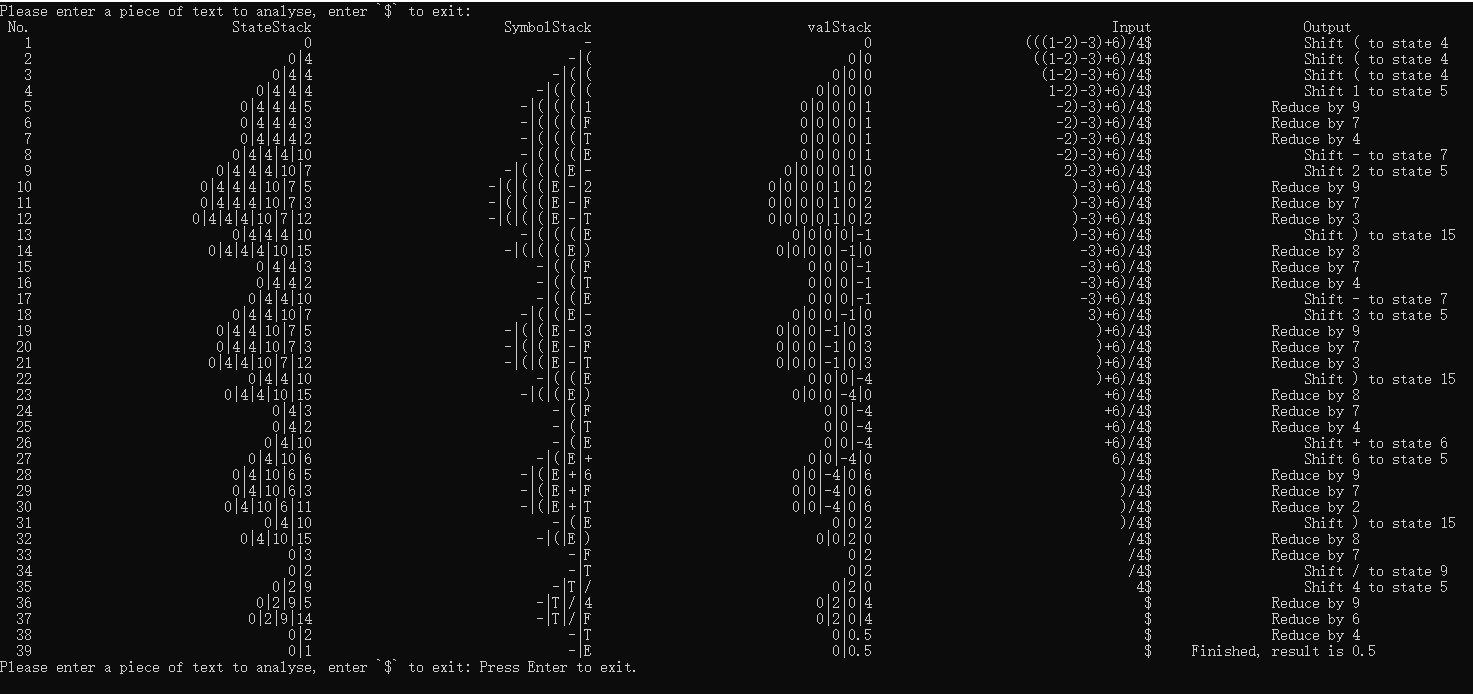
\includegraphics[width=\textwidth]{sample_3}
\begin{lstlisting}
Please enter a piece of text to analyse, enter `$` to exit:
 No.                         StateStack                        SymbolStack                           valStack                              Input                   Output
   1                                  0                                  -                                  0                   (((1-2)-3)+6)/4$                   Shift ( to state 4
   2                                0|4                                -|(                                0|0                    ((1-2)-3)+6)/4$                   Shift ( to state 4
   3                              0|4|4                              -|(|(                              0|0|0                     (1-2)-3)+6)/4$                   Shift ( to state 4
   4                            0|4|4|4                            -|(|(|(                            0|0|0|0                      1-2)-3)+6)/4$                   Shift 1 to state 5
   5                          0|4|4|4|5                          -|(|(|(|1                          0|0|0|0|1                       -2)-3)+6)/4$               Reduce by 9
   6                          0|4|4|4|3                          -|(|(|(|F                          0|0|0|0|1                       -2)-3)+6)/4$               Reduce by 7
   7                          0|4|4|4|2                          -|(|(|(|T                          0|0|0|0|1                       -2)-3)+6)/4$               Reduce by 4
   8                         0|4|4|4|10                          -|(|(|(|E                          0|0|0|0|1                       -2)-3)+6)/4$                   Shift - to state 7
   9                       0|4|4|4|10|7                        -|(|(|(|E|-                        0|0|0|0|1|0                        2)-3)+6)/4$                   Shift 2 to state 5
  10                     0|4|4|4|10|7|5                      -|(|(|(|E|-|2                      0|0|0|0|1|0|2                         )-3)+6)/4$               Reduce by 9
  11                     0|4|4|4|10|7|3                      -|(|(|(|E|-|F                      0|0|0|0|1|0|2                         )-3)+6)/4$               Reduce by 7
  12                    0|4|4|4|10|7|12                      -|(|(|(|E|-|T                      0|0|0|0|1|0|2                         )-3)+6)/4$               Reduce by 3
  13                         0|4|4|4|10                          -|(|(|(|E                         0|0|0|0|-1                         )-3)+6)/4$                   Shift ) to state 15
  14                      0|4|4|4|10|15                        -|(|(|(|E|)                       0|0|0|0|-1|0                          -3)+6)/4$               Reduce by 8
  15                            0|4|4|3                            -|(|(|F                           0|0|0|-1                          -3)+6)/4$               Reduce by 7
  16                            0|4|4|2                            -|(|(|T                           0|0|0|-1                          -3)+6)/4$               Reduce by 4
  17                           0|4|4|10                            -|(|(|E                           0|0|0|-1                          -3)+6)/4$                   Shift - to state 7
  18                         0|4|4|10|7                          -|(|(|E|-                         0|0|0|-1|0                           3)+6)/4$                   Shift 3 to state 5
  19                       0|4|4|10|7|5                        -|(|(|E|-|3                       0|0|0|-1|0|3                            )+6)/4$               Reduce by 9
  20                       0|4|4|10|7|3                        -|(|(|E|-|F                       0|0|0|-1|0|3                            )+6)/4$               Reduce by 7
  21                      0|4|4|10|7|12                        -|(|(|E|-|T                       0|0|0|-1|0|3                            )+6)/4$               Reduce by 3
  22                           0|4|4|10                            -|(|(|E                           0|0|0|-4                            )+6)/4$                   Shift ) to state 15
  23                        0|4|4|10|15                          -|(|(|E|)                         0|0|0|-4|0                             +6)/4$               Reduce by 8
  24                              0|4|3                              -|(|F                             0|0|-4                             +6)/4$               Reduce by 7
  25                              0|4|2                              -|(|T                             0|0|-4                             +6)/4$               Reduce by 4
  26                             0|4|10                              -|(|E                             0|0|-4                             +6)/4$                   Shift + to state 6
  27                           0|4|10|6                            -|(|E|+                           0|0|-4|0                              6)/4$                   Shift 6 to state 5
  28                         0|4|10|6|5                          -|(|E|+|6                         0|0|-4|0|6                               )/4$               Reduce by 9
  29                         0|4|10|6|3                          -|(|E|+|F                         0|0|-4|0|6                               )/4$               Reduce by 7
  30                        0|4|10|6|11                          -|(|E|+|T                         0|0|-4|0|6                               )/4$               Reduce by 2
  31                             0|4|10                              -|(|E                              0|0|2                               )/4$                   Shift ) to state 15
  32                          0|4|10|15                            -|(|E|)                            0|0|2|0                                /4$               Reduce by 8
  33                                0|3                                -|F                                0|2                                /4$               Reduce by 7
  34                                0|2                                -|T                                0|2                                /4$                   Shift / to state 9
  35                              0|2|9                              -|T|/                              0|2|0                                 4$                   Shift 4 to state 5
  36                            0|2|9|5                            -|T|/|4                            0|2|0|4                                  $               Reduce by 9
  37                           0|2|9|14                            -|T|/|F                            0|2|0|4                                  $               Reduce by 6
  38                                0|2                                -|T                              0|0.5                                  $               Reduce by 4
  39                                0|1                                -|E                              0|0.5                                  $     Finished, result is 0.5
Please enter a piece of text to analyse, enter `$` to exit: Press Enter to exit.
    \end{lstlisting}

\subsection{括号嵌套测试样例集:$sample\_4.txt$}
\begin{lstlisting}
( ( 89 - 34 ) + ( 22 - 10 ) ) / 20

    \end{lstlisting}
将$sample\_4.txt$文件拖拽至$main.exe$文件上,分析输出: \\
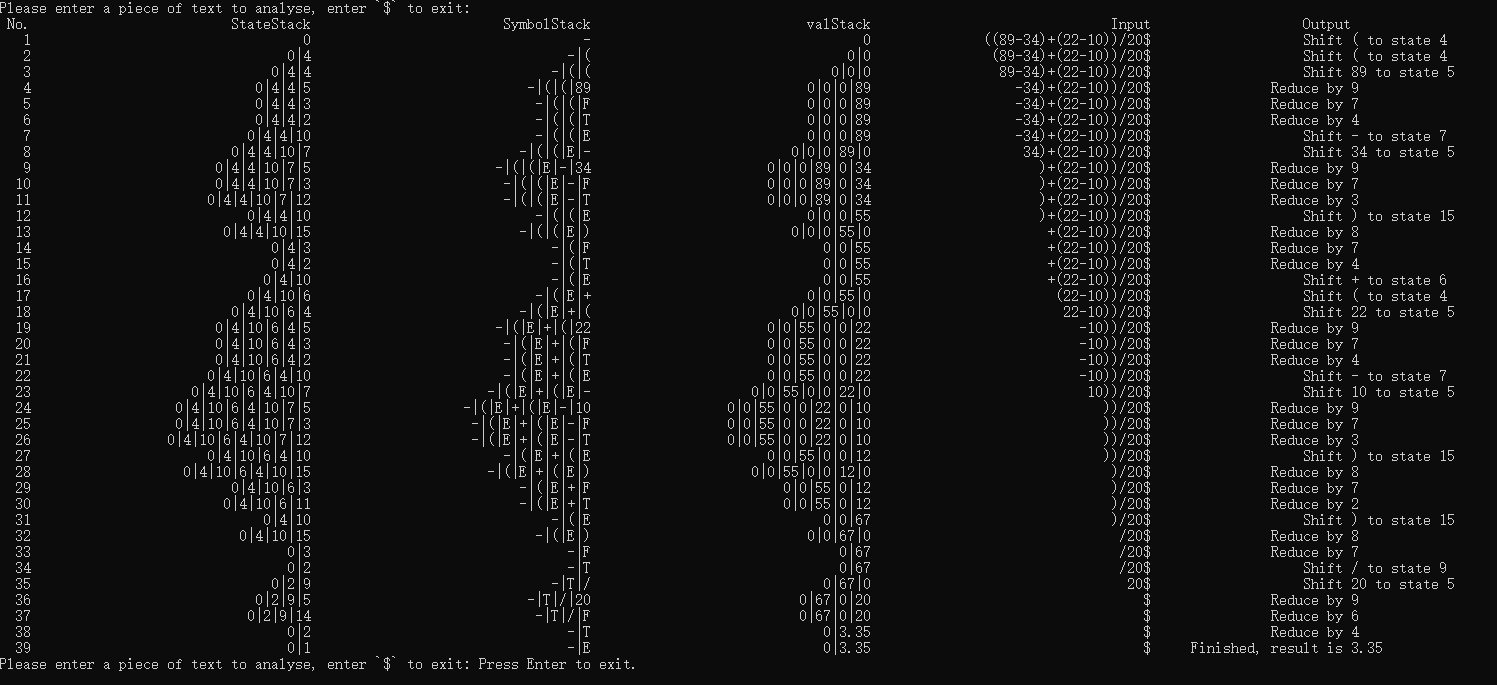
\includegraphics[width=\textwidth]{sample_4}
\begin{lstlisting}
Please enter a piece of text to analyse, enter `$` to exit:
 No.                         StateStack                        SymbolStack                           valStack                              Input                   Output
   1                                  0                                  -                                  0              ((89-34)+(22-10))/20$                   Shift ( to state 4
   2                                0|4                                -|(                                0|0               (89-34)+(22-10))/20$                   Shift ( to state 4
   3                              0|4|4                              -|(|(                              0|0|0                89-34)+(22-10))/20$                   Shift 89 to state 5
   4                            0|4|4|5                           -|(|(|89                           0|0|0|89                  -34)+(22-10))/20$               Reduce by 9
   5                            0|4|4|3                            -|(|(|F                           0|0|0|89                  -34)+(22-10))/20$               Reduce by 7
   6                            0|4|4|2                            -|(|(|T                           0|0|0|89                  -34)+(22-10))/20$               Reduce by 4
   7                           0|4|4|10                            -|(|(|E                           0|0|0|89                  -34)+(22-10))/20$                   Shift - to state 7
   8                         0|4|4|10|7                          -|(|(|E|-                         0|0|0|89|0                   34)+(22-10))/20$                   Shift 34 to state 5
   9                       0|4|4|10|7|5                       -|(|(|E|-|34                      0|0|0|89|0|34                     )+(22-10))/20$               Reduce by 9
  10                       0|4|4|10|7|3                        -|(|(|E|-|F                      0|0|0|89|0|34                     )+(22-10))/20$               Reduce by 7
  11                      0|4|4|10|7|12                        -|(|(|E|-|T                      0|0|0|89|0|34                     )+(22-10))/20$               Reduce by 3
  12                           0|4|4|10                            -|(|(|E                           0|0|0|55                     )+(22-10))/20$                   Shift ) to state 15
  13                        0|4|4|10|15                          -|(|(|E|)                         0|0|0|55|0                      +(22-10))/20$               Reduce by 8
  14                              0|4|3                              -|(|F                             0|0|55                      +(22-10))/20$               Reduce by 7
  15                              0|4|2                              -|(|T                             0|0|55                      +(22-10))/20$               Reduce by 4
  16                             0|4|10                              -|(|E                             0|0|55                      +(22-10))/20$                   Shift + to state 6
  17                           0|4|10|6                            -|(|E|+                           0|0|55|0                       (22-10))/20$                   Shift ( to state 4
  18                         0|4|10|6|4                          -|(|E|+|(                         0|0|55|0|0                        22-10))/20$                   Shift 22 to state 5
  19                       0|4|10|6|4|5                       -|(|E|+|(|22                      0|0|55|0|0|22                          -10))/20$               Reduce by 9
  20                       0|4|10|6|4|3                        -|(|E|+|(|F                      0|0|55|0|0|22                          -10))/20$               Reduce by 7
  21                       0|4|10|6|4|2                        -|(|E|+|(|T                      0|0|55|0|0|22                          -10))/20$               Reduce by 4
  22                      0|4|10|6|4|10                        -|(|E|+|(|E                      0|0|55|0|0|22                          -10))/20$                   Shift - to state 7
  23                    0|4|10|6|4|10|7                      -|(|E|+|(|E|-                    0|0|55|0|0|22|0                           10))/20$                   Shift 10 to state 5
  24                  0|4|10|6|4|10|7|5                   -|(|E|+|(|E|-|10                 0|0|55|0|0|22|0|10                             ))/20$               Reduce by 9
  25                  0|4|10|6|4|10|7|3                    -|(|E|+|(|E|-|F                 0|0|55|0|0|22|0|10                             ))/20$               Reduce by 7
  26                 0|4|10|6|4|10|7|12                    -|(|E|+|(|E|-|T                 0|0|55|0|0|22|0|10                             ))/20$               Reduce by 3
  27                      0|4|10|6|4|10                        -|(|E|+|(|E                      0|0|55|0|0|12                             ))/20$                   Shift ) to state 15
  28                   0|4|10|6|4|10|15                      -|(|E|+|(|E|)                    0|0|55|0|0|12|0                              )/20$               Reduce by 8
  29                         0|4|10|6|3                          -|(|E|+|F                        0|0|55|0|12                              )/20$               Reduce by 7
  30                        0|4|10|6|11                          -|(|E|+|T                        0|0|55|0|12                              )/20$               Reduce by 2
  31                             0|4|10                              -|(|E                             0|0|67                              )/20$                   Shift ) to state 15
  32                          0|4|10|15                            -|(|E|)                           0|0|67|0                               /20$               Reduce by 8
  33                                0|3                                -|F                               0|67                               /20$               Reduce by 7
  34                                0|2                                -|T                               0|67                               /20$                   Shift / to state 9
  35                              0|2|9                              -|T|/                             0|67|0                                20$                   Shift 20 to state 5
  36                            0|2|9|5                           -|T|/|20                          0|67|0|20                                  $               Reduce by 9
  37                           0|2|9|14                            -|T|/|F                          0|67|0|20                                  $               Reduce by 6
  38                                0|2                                -|T                             0|3.35                                  $               Reduce by 4
  39                                0|1                                -|E                             0|3.35                                  $     Finished, result is 3.35
Please enter a piece of text to analyse, enter `$` to exit: Press Enter to exit.
    \end{lstlisting}

\subsection{大数测试样例集:$sample\_5.txt$}
\begin{lstlisting}
( ( 12131 - 5442352 ) + 232 ) - ( 543252 - 536 ) / 4646

    \end{lstlisting}
将$sample\_5.txt$文件拖拽至$main.exe$文件上,分析输出: \\
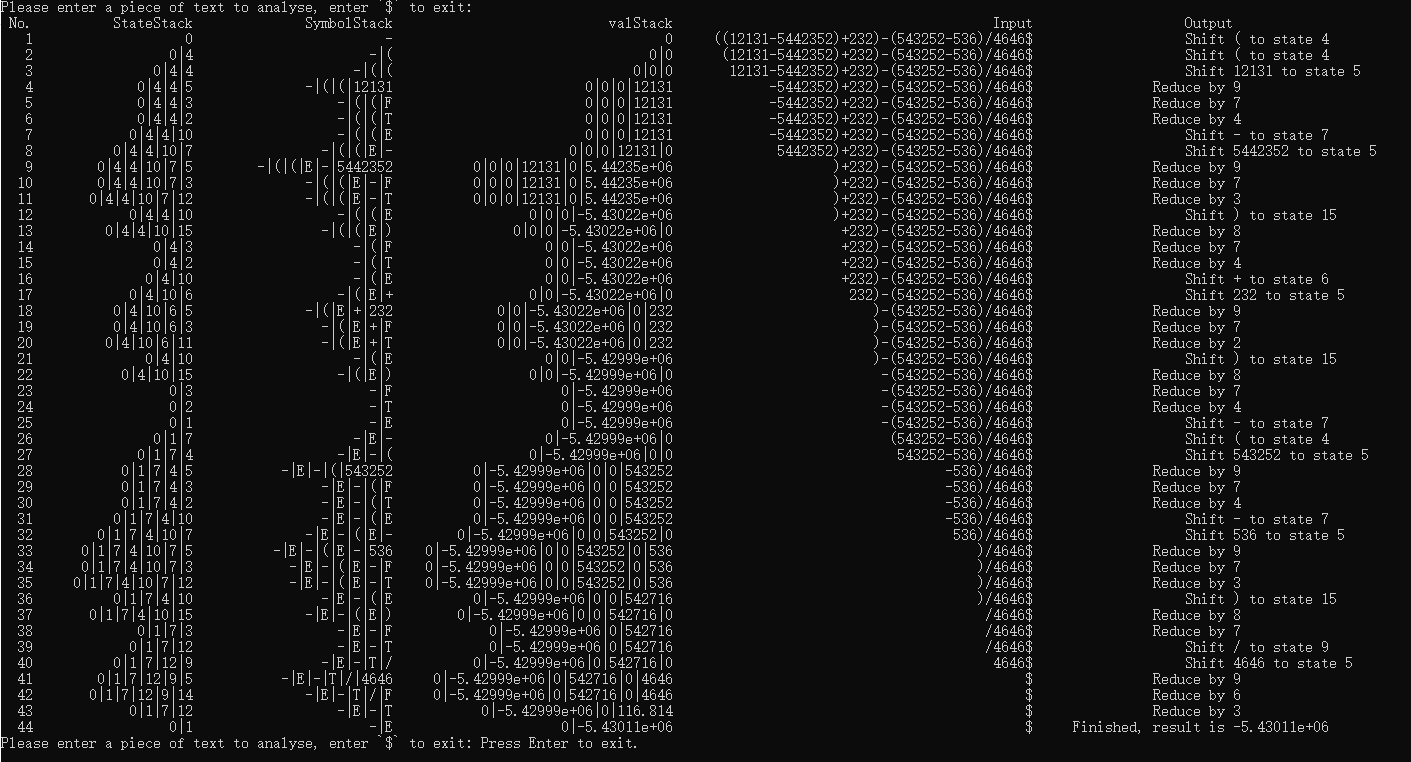
\includegraphics[width=\textwidth]{sample_5}
\begin{lstlisting}
Please enter a piece of text to analyse, enter `$` to exit:
 No.          StateStack              SymbolStack                           valStack                                        Input                   Output
   1                   0                        -                                  0     ((12131-5442352)+232)-(543252-536)/4646$                   Shift ( to state 4
   2                 0|4                      -|(                                0|0      (12131-5442352)+232)-(543252-536)/4646$                   Shift ( to state 4
   3               0|4|4                    -|(|(                              0|0|0       12131-5442352)+232)-(543252-536)/4646$                   Shift 12131 to state 5
   4             0|4|4|5              -|(|(|12131                        0|0|0|12131            -5442352)+232)-(543252-536)/4646$               Reduce by 9
   5             0|4|4|3                  -|(|(|F                        0|0|0|12131            -5442352)+232)-(543252-536)/4646$               Reduce by 7
   6             0|4|4|2                  -|(|(|T                        0|0|0|12131            -5442352)+232)-(543252-536)/4646$               Reduce by 4
   7            0|4|4|10                  -|(|(|E                        0|0|0|12131            -5442352)+232)-(543252-536)/4646$                   Shift - to state 7
   8          0|4|4|10|7                -|(|(|E|-                      0|0|0|12131|0             5442352)+232)-(543252-536)/4646$                   Shift 5442352 to state 5
   9        0|4|4|10|7|5        -|(|(|E|-|5442352          0|0|0|12131|0|5.44235e+06                    )+232)-(543252-536)/4646$               Reduce by 9
  10        0|4|4|10|7|3              -|(|(|E|-|F          0|0|0|12131|0|5.44235e+06                    )+232)-(543252-536)/4646$               Reduce by 7
  11       0|4|4|10|7|12              -|(|(|E|-|T          0|0|0|12131|0|5.44235e+06                    )+232)-(543252-536)/4646$               Reduce by 3
  12            0|4|4|10                  -|(|(|E                 0|0|0|-5.43022e+06                    )+232)-(543252-536)/4646$                   Shift ) to state 15
  13         0|4|4|10|15                -|(|(|E|)               0|0|0|-5.43022e+06|0                     +232)-(543252-536)/4646$               Reduce by 8
  14               0|4|3                    -|(|F                   0|0|-5.43022e+06                     +232)-(543252-536)/4646$               Reduce by 7
  15               0|4|2                    -|(|T                   0|0|-5.43022e+06                     +232)-(543252-536)/4646$               Reduce by 4
  16              0|4|10                    -|(|E                   0|0|-5.43022e+06                     +232)-(543252-536)/4646$                   Shift + to state 6
  17            0|4|10|6                  -|(|E|+                 0|0|-5.43022e+06|0                      232)-(543252-536)/4646$                   Shift 232 to state 5
  18          0|4|10|6|5              -|(|E|+|232             0|0|-5.43022e+06|0|232                         )-(543252-536)/4646$               Reduce by 9
  19          0|4|10|6|3                -|(|E|+|F             0|0|-5.43022e+06|0|232                         )-(543252-536)/4646$               Reduce by 7
  20         0|4|10|6|11                -|(|E|+|T             0|0|-5.43022e+06|0|232                         )-(543252-536)/4646$               Reduce by 2
  21              0|4|10                    -|(|E                   0|0|-5.42999e+06                         )-(543252-536)/4646$                   Shift ) to state 15
  22           0|4|10|15                  -|(|E|)                 0|0|-5.42999e+06|0                          -(543252-536)/4646$               Reduce by 8
  23                 0|3                      -|F                     0|-5.42999e+06                          -(543252-536)/4646$               Reduce by 7
  24                 0|2                      -|T                     0|-5.42999e+06                          -(543252-536)/4646$               Reduce by 4
  25                 0|1                      -|E                     0|-5.42999e+06                          -(543252-536)/4646$                   Shift - to state 7
  26               0|1|7                    -|E|-                   0|-5.42999e+06|0                           (543252-536)/4646$                   Shift ( to state 4
  27             0|1|7|4                  -|E|-|(                 0|-5.42999e+06|0|0                            543252-536)/4646$                   Shift 543252 to state 5
  28           0|1|7|4|5           -|E|-|(|543252          0|-5.42999e+06|0|0|543252                                  -536)/4646$               Reduce by 9
  29           0|1|7|4|3                -|E|-|(|F          0|-5.42999e+06|0|0|543252                                  -536)/4646$               Reduce by 7
  30           0|1|7|4|2                -|E|-|(|T          0|-5.42999e+06|0|0|543252                                  -536)/4646$               Reduce by 4
  31          0|1|7|4|10                -|E|-|(|E          0|-5.42999e+06|0|0|543252                                  -536)/4646$                   Shift - to state 7
  32        0|1|7|4|10|7              -|E|-|(|E|-        0|-5.42999e+06|0|0|543252|0                                   536)/4646$                   Shift 536 to state 5
  33      0|1|7|4|10|7|5          -|E|-|(|E|-|536    0|-5.42999e+06|0|0|543252|0|536                                      )/4646$               Reduce by 9
  34      0|1|7|4|10|7|3            -|E|-|(|E|-|F    0|-5.42999e+06|0|0|543252|0|536                                      )/4646$               Reduce by 7
  35     0|1|7|4|10|7|12            -|E|-|(|E|-|T    0|-5.42999e+06|0|0|543252|0|536                                      )/4646$               Reduce by 3
  36          0|1|7|4|10                -|E|-|(|E          0|-5.42999e+06|0|0|542716                                      )/4646$                   Shift ) to state 15
  37       0|1|7|4|10|15              -|E|-|(|E|)        0|-5.42999e+06|0|0|542716|0                                       /4646$               Reduce by 8
  38             0|1|7|3                  -|E|-|F            0|-5.42999e+06|0|542716                                       /4646$               Reduce by 7
  39            0|1|7|12                  -|E|-|T            0|-5.42999e+06|0|542716                                       /4646$                   Shift / to state 9
  40          0|1|7|12|9                -|E|-|T|/          0|-5.42999e+06|0|542716|0                                        4646$                   Shift 4646 to state 5
  41        0|1|7|12|9|5           -|E|-|T|/|4646     0|-5.42999e+06|0|542716|0|4646                                            $               Reduce by 9
  42       0|1|7|12|9|14              -|E|-|T|/|F     0|-5.42999e+06|0|542716|0|4646                                            $               Reduce by 6
  43            0|1|7|12                  -|E|-|T           0|-5.42999e+06|0|116.814                                            $               Reduce by 3
  44                 0|1                      -|E                     0|-5.43011e+06                                            $     Finished, result is -5.43011e+06
Please enter a piece of text to analyse, enter `$` to exit: Press Enter to exit.
    \end{lstlisting}
\end{document}